\documentclass[12pt]{article}
\usepackage{graphicx}

\usepackage[margin=1in]{geometry}
\usepackage{listings}

\title{Labwork 2: GPU Information Report}
\author{Ngo Quang Truong 2540106}
\date{29 Sep 2026}

\begin{document}

\maketitle
\newpage

\section{Introduction}

This report describes a Python program used to obtain basic information
about available NVIDIA GPUs using the \texttt{Numba CUDA} interface.
The program identifies the active GPU and then iterates through all
available GPUs to collect hardware information.

\section{Method}

The program uses the following Numba CUDA functionality:

\begin{itemize}
    \item \texttt{cuda.get\_current\_device()} to identify the currently active GPU.
    \item \texttt{cuda.gpus} to iterate over all available GPUs.
    \item \texttt{MULTIPROCESSOR\_COUNT} to obtain the number of streaming multiprocessors (SMs).
    \item \texttt{compute\_capability} to obtain the GPU compute capability.
    \item \texttt{get\_memory\_info()} to determine the available and total GPU memory.
\end{itemize}

\section{Output}

For each detected GPU, the program reports the following information:

\begin{table}[h]
\centering
\begin{tabular}{ll}
\hline
\textbf{Parameter} & \textbf{Description} \\
\hline
GPU ID & Identifier of the GPU device \\
Name & Model name of the GPU \\
SM Count & Number of streaming multiprocessors \\
Compute Capability & CUDA compute capability version \\
Estimated CUDA Cores & Estimated number of CUDA cores \\
Total Memory & Total GPU memory in GB and bytes \\
\hline
\end{tabular}
\caption{GPU information collected by the program}
\end{table}

\begin{figure}[h]
    \centering
    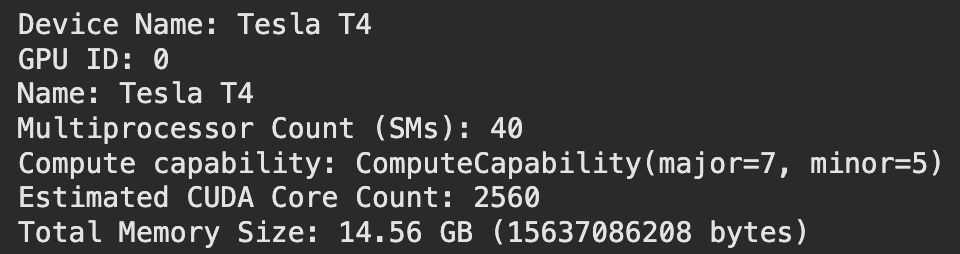
\includegraphics[width=0.9\textwidth]{gpu_output.png}
    \caption{Output of the GPU information program}
    \label{fig:gpu-output}
\end{figure}

\end{document}